\section{Graphics}
On figur \ref{fig:test-graph} you see a figure displaying common features of a graph
\begin{figure}[h]
\centering
\caption{Look, this caption is above the image!}
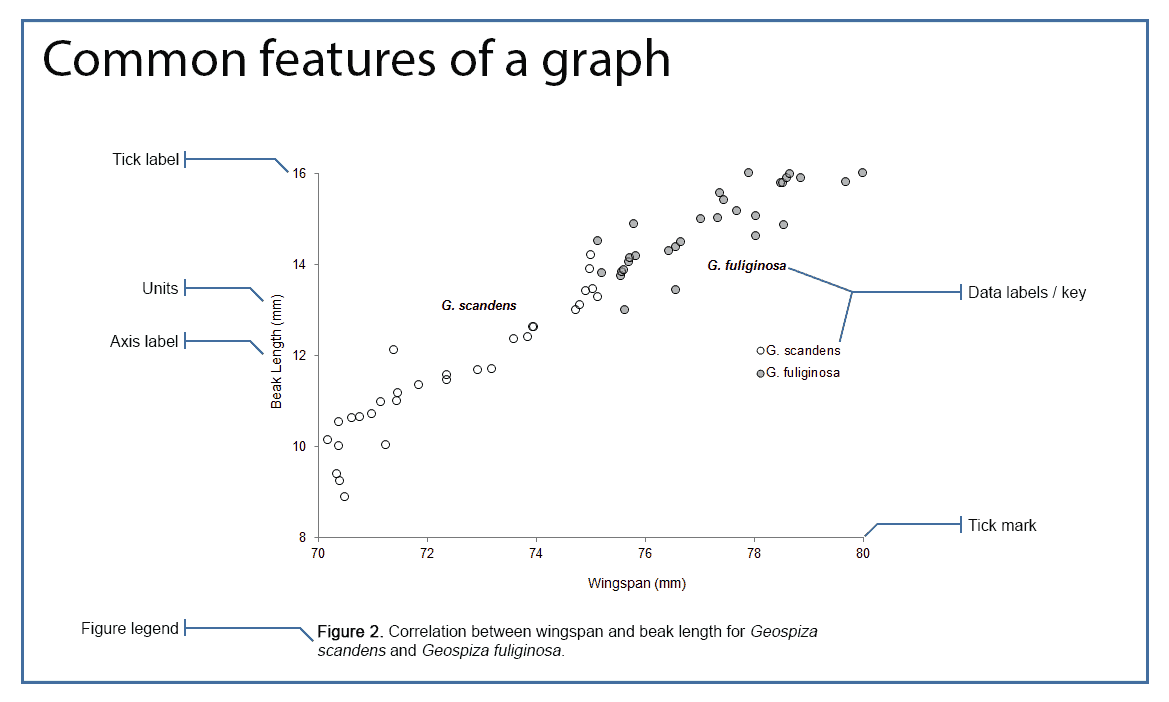
\includegraphics[scale=0.35]{/graphs/graph01.png}
\caption{This is just an example graph}
\label{fig:test-graph}
\end{figure}

Mauris ut ultrices augue. Vestibulum at tristique nibh. Pellentesque elit nibh, tincidunt at lorem nec, dignissim malesuada lorem. Donec tristique nisi vitae odio finibus, id tincidunt augue congue.

\begin{figure}
    \centering
    \begin{subfigure}[b]{0.3\textwidth}
        \centering
        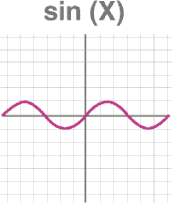
\includegraphics[width=\textwidth]{graphs/graph02.png}
        \caption{$sin(x)$}
        \label{fig:sin(x)}
    \end{subfigure}
    \hfill % hfill will add space between the figures %
    \begin{subfigure}[b]{0.3\textwidth}
        \centering
        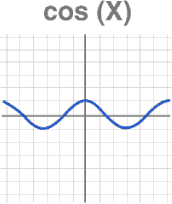
\includegraphics[width=\textwidth]{graphs/graph03.png}
        \caption{$cos(x)$}
        \label{fig:cos(x)}
    \end{subfigure}
    \hfill % hfill will add space between the figures %
    \begin{subfigure}[b]{0.3\textwidth}
        \centering
        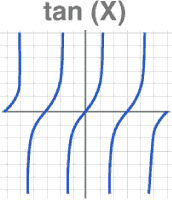
\includegraphics[width=\textwidth]{graphs/graph04.png}
        \caption{$tan(x)$}
        \label{fig:tan(x)}
    \end{subfigure}
    \caption{Three sample graphs (i added a third image for extra flair)}
    \label{fig: three graphs}
\end{figure}

Sed varius diam risus, ut condimentum nibh bibendum nec. Lorem ipsum dolor sit amet, consectetur adipiscing elit. Morbi aliquam lectus congue, porttitor erat eu, malesuada quam. Cras facilisis tellus eu euismod efficitur. Aliquam eget imperdiet est, faucibus egestas ligula.\\